\item \textbf{Sylvester 恒等式（Sylvester identity）}是一条联系向量化、矩阵乘法与 Kronecker 积的非常有用的恒等式：$$\vectorize(\Ab\Xb\Bb) = (\Ab\kron \Bb^\ts)\vectorize(\Xb),$$
其中 $\Ab\in\RR^{m\times n},\Xb\in\RR^{n\times p}$ 且 $\Bb\in\RR^{p\times q}.$
\begin{proof}
利用张量网络，证明相当直接： 
\begin{align*}
\vectorize(\Ab\Xb\Bb) &=
 \vectorize\left(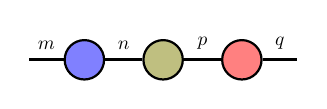
\begin{tikzpicture}[baseline=-0.5ex]
    \tikzset{tensor/.style = {minimum size = 0.5cm,shape = circle,thick,draw=black,inner sep = 0pt}, edge/.style = {thick,line width=.4mm},every loop/.style={}}
    \def\x{6}
    \node[tensor,fill=blue!50!white] (A) at (\x-1,0) {$\Ab$};
    \node[tensor,fill=green!50!red!50!white] (X) at (\x,0) {$\Xb$};
    \node[tensor,fill=red!50!white] (B) at (\x+1,0) {$\Bb$};
    \draw[edge] (A) -- (X) node [midway,above] {\scalebox{0.7}{\dimcolor{$n$}}};
    \draw[edge] (X) -- (B) node [midway,above] {\scalebox{0.7}{\dimcolor{$p$}}};
    \draw[edge] (A) -- (\x-1.7,0) node [midway,above] {\scalebox{0.7}{\dimcolor{$m$}}};
    \draw[edge] (B) -- (\x+1.7,0) node [midway,above] {\scalebox{0.7}{\dimcolor{$q$}}};
    \end{tikzpicture}\right)
=
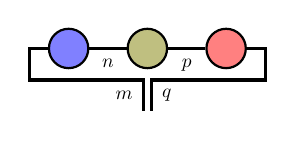
\begin{tikzpicture}[baseline=-0.5ex]
    \tikzset{tensor/.style = {minimum size = 0.5cm,shape = circle,thick,draw=black,inner sep = 0pt}, edge/.style = {thick,line width=.4mm},every loop/.style={}}
    \def\x{6}
    \node[tensor,fill=blue!50!white] (A) at (\x-1,0) {$\Ab$};
    \node[tensor,fill=green!50!red!50!white] (X) at (\x,0) {$\Xb$};
    \node[tensor,fill=red!50!white] (B) at (\x+1,0) {$\Bb$};
    \draw[edge] (A) -- (X) node [midway,below] {\scalebox{0.7}{\dimcolor{$n$}}};
    \draw[edge] (X) -- (B) node [midway,below] {\scalebox{0.7}{\dimcolor{$p$}}};
    \draw[edge] (A) -- (\x-1.5,0) -- (\x-1.5,-0.4) -- (\x-0.05,-0.4)--(\x-0.05,-0.8) node [midway,left] {\scalebox{0.7}{\dimcolor{$m$}}};
    \draw[edge] (B) -- (\x+1.5,0) -- (\x+1.5,-0.4) -- (\x+0.05,-0.4)--(\x+0.05,-0.8) node [midway,right] {\scalebox{0.7}{\dimcolor{$q$}}};
\end{tikzpicture}\\
&=
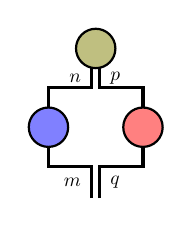
\begin{tikzpicture}[baseline=-2ex]
    \tikzset{tensor/.style = {minimum size = 0.5cm,shape = circle,thick,draw=black,inner sep = 0pt}, edge/.style = {thick,line width=.4mm},every loop/.style={}}
    \def\x{6}
    \draw[edge] (\x-0.05,0.25) -- (\x-0.05,0) node [midway, left] {\scalebox{0.7}{\dimcolor{$n$}}}   -- (\x-0.6,0) -- (\x-0.6,-0.25) ; 
    \draw[edge] (\x+0.05,0.25) -- (\x+0.05,0)   node [midway, right] {\scalebox{0.7}{\dimcolor{$p$}}}  -- (\x+0.6,0) -- (\x+0.6,-0.25);    
    \draw[edge] (\x-0.05,-1.4) -- (\x-0.05,-1)  node [midway, left] {\scalebox{0.7}{\dimcolor{$m$}}}  -- (\x-0.6,-1) -- (\x-0.6,-0.75) ; 
    \draw[edge] (\x+0.05,-1.4) -- (\x+0.05,-1)  node [midway, right] {\scalebox{0.7}{\dimcolor{$q$}}}   -- (\x+0.6,-1) -- (\x+0.6,-0.75); 
     \node[tensor,fill=green!50!red!50!white] (X) at (\x,0.5) {$\Xb$};
    \node[tensor,fill=blue!50!white] (A) at (\x-0.6,-0.5) {$\Ab$};
    \node[tensor,fill=red!50!white] (B) at (\x+0.6,-0.5) {$\Bb$};
\end{tikzpicture}
=
(\Ab\kron\Bb^\ts)\vectorize(\Xb).
\end{align*}
在最后一个图中，容易看出 $\Xb$ 的向量化以及 $\Ab$ 与 $\Bb$ 的 Kronecker 积，从而可以断定该张量网络表示二者之间的矩阵-向量乘法。然而，把张量网络翻译成经典数学记法时需要注意一些细节。首先，由于 $\vectorize(\Xb)$ 的维度为 $np$，Kronecker 积必须取在 $\Ab$ 与 $\Bb^\ts$ 之间，才能得到形状为 $mq\times np$ 的矩阵。其次，需要确定使用哪一个 Kronecker 积：$\Ab \kron \Bb^\ts$ 还是 $\Bb^\ts \kron \Ab$，二者的形状都正确。由于本手稿对 $\vectorize$ 这类重排运算采用字典序，正确的写法是  $\Ab \kron \Bb^\ts$。然而，若采用逆字典序，如~\citep{kolda2009tensor} 中的做法，正确的写法应为 $\Bb^\ts \kron \Ab$。
\end{proof}
\emph{Sylvester 恒等式}是求解形如 $\Ab\Xb+\Xb\Bb = \Cb$ 的方程组的有用恒等式。
\end{enumerate}
\end{remark}
模 $n$ 乘积、矩阵化与 Kronecker 积之间存在若干有用的关系： 
\begin{proposition}
设 $\Tt\in\RR^{d_1\times d_2\times\dots\times d_p}$，$\Ab_1\in\RR^{d_1\times n_1},
\Ab_2\in\RR^{d_2\times n_2},\dots,$
$\Ab_p\in\RR^{d_p\times n_p}$，则 
\begin{align*}(\Tt\ttm1\Ab_1\ttm2\Ab_2\ttm3\Ab_3\ttm4\dots\ttm p\Ab_p)_{(n)}=
\Ab_n\Tt_{(n)}(\Ab_1\kron\dots\kron\Ab_{n-1}\kron\Ab_{n+1}\kron\dots\kron\Ab_p)^\ts.
\end{align*}
\end{proposition}
\begin{proof}
当 $p =3$ 且 $n=1$ 时，
\begin{align*}
(\Tt\ttm1\Ab_1\ttm2\Ab_2\ttm3\Ab_3)_{(1)}
&= 
 \left(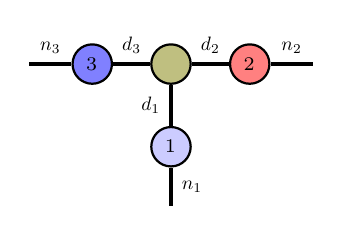
\begin{tikzpicture}[baseline=-0.5ex]
    \tikzset{tensor/.style = {minimum size = 0.5cm,shape = circle,thick,draw=black,inner sep = 0pt}, edge/.style = {thick,line width=.4mm},every loop/.style={}}
    \def\x{6}
    \node[tensor,fill=blue!20!white] (A1) at (\x,-1.05) {$\Ab_1$};
    \node[tensor,fill=green!50!red!50!white] (At) at (\x,0) {$\Tt$};
    \node[tensor,fill=red!50!white] (A2) at (\x+1,0) {$\Ab_2$};
    \node[tensor,fill=blue!50!white] (A3) at (\x-1,0) {$\Ab_3$};
    \draw[edge] (At) -- (A2) node [midway,above] {\scalebox{0.7}{\dimcolor{$d_2$}}};
    \draw[edge] (At) -- (A1) node [midway,left] {\scalebox{0.7}{\dimcolor{$d_1$}}};
    \draw[edge] (At) -- (A3) node [midway,above] {\scalebox{0.7}{\dimcolor{$d_3$}}};
    \draw[edge] (A1) -- (\x,-1.8) node [midway,right] {\scalebox{0.7}{\dimcolor{$n_1$}}};
    \draw[edge] (A2) -- (\x+1.8,0) node [midway,above] {\scalebox{0.7}{\dimcolor{$n_2$}}};
    \draw[edge] (A3) -- (\x-1.8,0) node [midway,above] {\scalebox{0.7}{\dimcolor{$n_3$}}};
    \end{tikzpicture}\right)_{(1)}
=
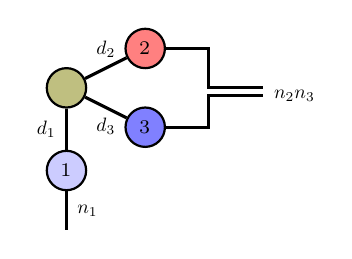
\begin{tikzpicture}[baseline=-0.5ex]
    \tikzset{tensor/.style = {minimum size = 0.5cm,shape = circle,thick,draw=black,inner sep = 0pt}, edge/.style = {thick,line width=.4mm},every loop/.style={}}
    \def\x{6}
    \def\y{0}
    \node[tensor,fill=blue!20!white] (A1) at (\x,-1.05) {$\Ab_1$};
    \node[tensor,fill=green!50!red!50!white] (At) at (\x,0) {$\Tt$};
    \node[tensor,fill=red!50!white] (A2) at (\x+1,\y+0.5) {$\Ab_2$};
    \node[tensor,fill=blue!50!white] (A3) at (\x+1,\y-0.5) {$\Ab_3$};
    \draw[edge] (At) -- (A1) node [midway,left] {\scalebox{0.7}{\dimcolor{$d_1$}}};
    \draw[edge] (At) -- (A3) node [midway,below] {\scalebox{0.7}{\dimcolor{$d_3$}}};
    \draw[edge] (At) -- (A2) node [midway,above] {\scalebox{0.7}{\dimcolor{$d_2$}}};
    \draw[edge] (A1) -- (\x,-1.8) node [midway,right] {\scalebox{0.7}{\dimcolor{$n_1$}}};
    \draw[edge] (A2) -- (\x+1.8,\y+0.5) -- (\x+1.8,\y)-- (\x+2.5,\y);
    \draw[edge] (A3) -- (\x+1.8,\y-0.5) -- (\x+1.8,\y-0.1) -- (\x+2.5,\y-0.1)node [right] {\scalebox{0.7}{\dimcolor{$n_2n_3$}}};
    \end{tikzpicture}\\
&=
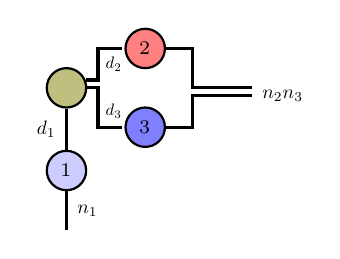
\begin{tikzpicture}[baseline=-0.5ex]
    \tikzset{tensor/.style = {minimum size = 0.5cm,shape = circle,thick,draw=black,inner sep = 0pt}, edge/.style = {thick,line width=.4mm},every loop/.style={}}
    \def\x{6}
    \def\y{0}
    \node[tensor,fill=blue!20!white] (A1) at (\x,-1.05) {$\Ab_1$};
    \node[tensor,fill=green!50!red!50!white] (At) at (\x,0) {$\Tt$};
    \node[tensor,fill=red!50!white] (A2) at (\x+1,\y+0.5) {$\Ab_2$};
    \node[tensor,fill=blue!50!white] (A3) at (\x+1,\y-0.5) {$\Ab_3$};
    \draw[edge] (At) -- (A1) node [midway,left] {\scalebox{0.7}{\dimcolor{$d_1$}}};
    \draw[edge] (\x+0.7,\y-0.5) -- (\x+0.4,\y-0.5) -- (\x+0.4,\y) -- (\x+0.25,\y);
    \draw[edge] (\x+0.7,\y+0.5) -- (\x+0.4,\y+0.5) -- (\x+0.4,\y+0.1) -- (\x+0.25,\y+0.1);
    \draw[edge] (A1) -- (\x,-1.8) node [midway,right] {\scalebox{0.7}{\dimcolor{$n_1$}}};
    \draw[edge] (A2) -- (\x+1.6,\y+0.5) -- (\x+1.6,\y)-- (\x+2.35,\y);
    \draw[edge] (A3) -- (\x+1.6,\y-0.5) -- (\x+1.6,\y-0.1) -- (\x+2.35,\y-0.1)node [right] {\scalebox{0.7}{\dimcolor{$n_2n_3$}}};
    \node[draw=none] () at (\x+0.6,\y-0.3) {\scalebox{0.6}{\dimcolor{$d_3$}}};
    \node[draw=none] () at (\x+0.6,\y+0.3) {\scalebox{0.6}{\dimcolor{$d_2$}}};
\end{tikzpicture}
=
\Ab_1\Tt_{(1)}(\Ab_2\kron\Ab_3)^\ts.
\end{align*}
\end{proof}
\begin{proposition}
    设 $\Tt\in\RR^{d_1\times d_2\times\cdots\times d_p}$  且对 $i\in[p]$ 有 $\Ab_i\in\RR^{d_i\times n_i}$。设 $m \in [p]$，
记 $\Tt_{([m])}$ 表示把张量 $\Tt$ 重排为尺寸 $d_1d_2\cdots d_m\times d_{m+1}...d_p$ 的矩阵：前 $m$ 个指标映射到
行，其余指标映射到列。于是，
\begin{align*}
    (\Tt\ttm 1\Ab_1\ttm 2 \Ab_2\cdots\ttm p \Ab_p)_{([m])}=(\Ab_1\kron\Ab_2\kron\cdots\kron\Ab_{m})\Tb_{([m])}(\Ab_{m+1}\kron\Ab_{m+2}\kron\cdots\kron\Ab_{p})^\ts.
\end{align*}
此恒等式可推广到任意子集 $I\subset [p]$：
$$ (\Tt\ttm 1\Ab_1\ttm 2 \Ab_2\cdots\ttm p \Ab_p)_{(I)}    = \left(\bigotimes_{i\in I} \Ab_i\right)\Tt_{([m])}\left(\bigotimes_{i\in [p] \setminus I} \Ab_i\right)^\ts.$$
\begin{proof}
当 $p=6$ 且 $I = \{1,2,3\}$ 时，
\begin{align*}
\left(\begin{tikzpicture}[baseline=\baseline]
    \tikzset{tensor/.style = {minimum size = 0.5cm,shape = circle,thick,draw=black,inner sep = 0pt}, edge/.style = {thick,line width=.4mm},every loop/.style={}}
    \def\y{0}
    \def\x{0}
    \node[tensor,fill=red!20!blue!40!white] (T) at (\x,\y){\scalebox{0.85}{$\Tt$}};
\node[tensor,fill=red!20!white] (A) at (\x+1,\y){\scalebox{0.85}{$\Ab_1$}};
    \draw[edge](T) -- (A) node [midway,above] {\scalebox{0.7}{\dimcolor{$d_1$}}};
    \draw[edge](A) -- (\x+2,\y) node [midway,above] {\scalebox{0.7}{\dimcolor{$n_1$}}};
\node[tensor,fill=red!40!white] (B) at (\x,\y-1) {\scalebox{0.85}{$\Ab_2$}}; 
    \draw[edge](T) -- (B) node [midway,left] {\scalebox{0.7}{\dimcolor{$d_2$}}};
    \draw[edge](B) -- (\x,\y-2) node [midway,left] {\scalebox{0.7}{\dimcolor{$n_2$}}};
\node[tensor,fill=red!60!white] (C) at (\x-1,\y) {\scalebox{0.85}{$\Ab_3$}};
    \draw[edge](T) -- (C) node [midway,above] {\scalebox{0.7}{\dimcolor{$d_3$}}};
    \draw[edge](C) -- (\x-2,\y) node [midway,above] {\scalebox{0.7}{\dimcolor{$n_3$}}};
\node[tensor,fill=blue!20!white] (D) at (\x,\y+1){\scalebox{0.85}{$\Ab_4$}}; 
    \draw[edge](T) -- (D) node [midway,right] {\scalebox{0.7}{\dimcolor{$d_4$}}};
    \draw[edge](D) -- (\x,\y+2) node [midway,right] {\scalebox{0.7}{\dimcolor{$n_4$}}};
\node[tensor,fill=red!50!blue!10!white] (E) at (\x-0.85,\y+0.85){\scalebox{0.85}{$\Ab_5$}}; 
   \draw[edge](T) -- (E) node [midway,above] {\scalebox{0.7}{\dimcolor{$d_5$}}};
    \draw[edge](E) -- (\x-1.5,\y+1.5) node [midway,right] {\scalebox{0.7}{\dimcolor{$n_5$}}};
\node[tensor,fill=blue!50!white] (F) at (\x+0.85,\y-0.85){\scalebox{0.85}{$\Ab_6$}};
    \draw[edge](T) -- (F)node [midway,right] {\scalebox{0.7}{\dimcolor{$d_6$}}};
    \draw[edge](F) -- (\x+1.5,\y-1.5)node [midway,right] {\scalebox{0.7}{\dimcolor{$n_6$}}};
\end{tikzpicture}\right)_{(\{1,2,3\})}
\begin{tikzpicture}[baseline=\baseline]
    \tikzset{tensor/.style = {minimum size = 0.5cm,shape = circle,thick,draw=black,inner sep = 0pt}, edge/.style = {thick,line width=.4mm},every loop/.style={}}
    \def\y{0}
    \def\x{0}
    \node[draw=none] at (\x-3.5,\y){$=$};
    \node[tensor,fill=red!20!blue!40!white] (T) at (\x,\y){\scalebox{0.85}{$\Tb$}};
    \node[tensor,fill=red!20!white] (A) at (\x-1.5,\y-1){\scalebox{0.85}{$\Ab_1$}};
    \node[tensor,fill=red!40!white] (B) at (\x-1.5,\y) {\scalebox{0.85}{$\Ab_2$}}; 
    \node[tensor,fill=red!60!white] (C) at (\x-1.5,\y+1) {\scalebox{0.85}{$\Ab_3$}};
    \node[tensor,fill=blue!20!white] (D) at (\x+1.5,\y-1){\scalebox{0.85}{$\Ab_4$}};
\node[tensor,fill=red!50!blue!10!white] (E) at (\x+1.5,\y){\scalebox{0.85}{$\Ab_5$}}; 
\node[tensor,fill=blue!50!white] (F) at (\x+1.5,\y+1){\scalebox{0.85}{$\Ab_6$}};
    \draw[edge](T) -- (B);
    \node[draw=none] at (\x-1.15,\y+0.2) {\scalebox{0.7}{\dimcolor{$d_2$}}};;
    \node[draw=none] at (\x+1.15,\y+0.2) {\scalebox{0.7}{\dimcolor{$d_5$}}};;
    \draw[edge](B) -- (\x-2.5,\y);;
    \draw[edge](\x+0.16,\y+0.2) -- (\x+0.5,\y+0.2) -- (\x+0.5,\y+0.1) -- (\x+1,\y+0.1);
    \draw[edge](F) -- (\x+1,\y+1) -- (\x+1,\y+0.1)node [midway,left] {\scalebox{0.7}{\dimcolor{$d_6$}}};
    \draw[edge](F) -- (\x+2,\y+1)--(\x+2,\y+0.1)-- (\x+2.5,\y+0.1)node [near end,above] {\scalebox{0.7}{\dimcolor{$n_6$}}};
    \draw[edge](\x+0.16,\y-0.2) -- (\x+0.5,\y-0.2) -- (\x+0.5,\y-0.1) -- (\x+1,\y-0.1);
    \draw[edge](D) -- (\x+1,\y-1) -- (\x+1,\y-0.1)node [midway,left] {\scalebox{0.7}{\dimcolor{$d_4$}}};
    \draw[edge](D) -- (\x+2,\y-1)--(\x+2,\y-0.1)-- (\x+2.5,\y-0.1)node [near end,below] {\scalebox{0.7}{\dimcolor{$n_4$}}};
    \draw[edge](T) -- (E);
    \draw[edge](E) -- (\x+2.5,\y);
    \draw[edge](\x-0.16,\y+0.2) -- (\x-0.5,\y+0.2) -- (\x-0.5,\y+0.1) -- (\x-1,\y+0.1);
    \draw[edge](C) -- (\x-1,\y+1) -- (\x-1,\y+0.1)node [midway,right] {\scalebox{0.7}{\dimcolor{$d_3$}}};
    \draw[edge](C) -- (\x-2,\y+1)--(\x-2,\y+0.1)-- (\x-2.5,\y+0.1)node [near end,above] {\scalebox{0.7}{\dimcolor{$n_3$}}};;;
    \draw[edge](\x-0.16,\y-0.2) -- (\x-0.5,\y-0.2) -- (\x-0.5,\y-0.1) -- (\x-1,\y-0.1);
    \draw[edge](A) --  (\x-2,\y-1)--(\x-2,\y-0.1)-- (\x-2.5,\y-0.1)node [near end,below] {\scalebox{0.7}{\dimcolor{$n_1$}}};;
    \draw[edge](A) -- (\x-1,\y-1) -- (\x-1,\y-0.1)node [midway,right] {\scalebox{0.7}{\dimcolor{$d_1$}}};
    \node[draw=none] at (\x+2.8,\y){\scalebox{0.7}{\dimcolor{$n_4$}}};
    \node[draw=none] at (\x-2.8,\y){\scalebox{0.7}{\dimcolor{$n_2$}}};
\end{tikzpicture}.
\end{align*}
\end{proof}
\end{proposition}

